\documentclass[unknownkeysallowed]{beamer}
\mode<presentation>
{
%  \usetheme{AnnArbor}
%  \usetheme{Dresden}
%  \usetheme{Montpellier}
%  \usetheme{Antibes}
%  \usetheme{Frankfurt}
%  \usetheme{PaloAlto}
%  \usetheme{Bergen}
%  \usetheme{Boadilla}
%  \usetheme{Goettingen}
%  \usetheme{Pittsburgh}	%!!
%  \usetheme{Berkeley}
%  \usetheme{Hannover}
%  \usetheme{Rochester}		%!!!
%  \usetheme{Berlin}
%  \usetheme{Ilmenau}
%  \usetheme{Singapore}
  \usetheme{Boadilla}		%viel platz
%  \usetheme{JuanLesPins}
%  \usetheme{Szeged}		%!
%  \usetheme{boxes}
%  \usetheme{Luebeck}
%  \usetheme{Warsaw}
%  \usetheme{Copenhagen}
%  \usetheme{Madrid}
%  \usetheme{Darmstadt}
%  \usetheme{Malmoe}
%  \usetheme{default}
%  \usetheme{JuanLesPins}

%  \usetheme{Marburg}


%\usefonttheme{professionalfonts}
%	default | professionalfonts | serif |
%	structurebold | structureitalicserif |
%	structuresmallcapsserif
%\useinnertheme{rounded}
%	circles | default | inmargin |
%	rectangles | rounded

%  \setbeamercovered{transparent}
  % oder auch nicht
\usecolortheme{rose}


\definecolor{uaf yellow}{cmyk}{0,0.16,1,0} % official UAF yellow
\definecolor{light yellow}{cmyk}{0.01,0,0.16,0}
\definecolor{uaf blue}{cmyk}{1,0.66,0,0.02} % official UAF blue
\definecolor{light blue}{cmyk}{0.22,0.11,0,0}
\definecolor{arsc blue}{HTML}{005496}
\definecolor{arsc red}{HTML}{a20a42}
\definecolor{arsc green}{HTML}{009a82}
\definecolor{light gray}{HTML}{777777}

  %navigation aus, klaut nur platz
  \setbeamertemplate{navigation symbols}{}
% Reset title background to default
%\setbeamertemplate{title page}[default]
\setbeamercolor{title}{bg=}
\setbeamercolor{frametitle}{bg=uaf blue, fg=white}
\setbeamercolor{institute}{fg=white}
\setbeamercolor{date}{fg=white}
\setbeamercolor{block}{bg=}
%\setbeamercolor{title}{fg=black}

% Reset block background to default
%\setbeamertemplate{blocks}[default]
%\setbeamercolor{block title}{bg=}
%\setbeamercolor{block body}{bg=}

\beamertemplatenavigationsymbolsempty  
\setbeamertemplate{blocks}[rounded][shadows=false]

\useinnertheme{circles}

}
\usepackage[latin1]{inputenc}
\usepackage{latexsym}
\usepackage{amsfonts}
%\usepackage{natbib}
\usepackage{fancyhdr}
\usepackage{graphicx}
%\usepackage{subfigure}
% oder was auch immer
\usepackage{grffile}
\usepackage{pgf}
\usepackage{tikz}

\usepackage{listings}

\usepackage{times}
\usepackage[T1]{fontenc}
%\usepackage{appendixnumber}
% Oder was auch immer. Zu beachten ist, das Font und Encoding passen
% m�ssen. Falls T1 nicht funktioniert, kann man versuchen, die Zeile
% mit fontenc zu l�schen.

\hypersetup{
    bookmarks=true,         % show bookmarks bar?
    unicode=false,          % non-Latin characters in Acrobat's bookmarks
    pdftoolbar=true,        % show Acrobat's toolbar?
    pdfmenubar=true,        % show Acrobat's menu?
    pdffitwindow=false,     % window fit to page when opened
    pdfstartview={FitH},    % fits the width of the page to the window
    pdftitle={My title},    % title
    pdfauthor={Author},     % author
    pdfsubject={Subject},   % subject of the document
    pdfcreator={Creator},   % creator of the document
    pdfproducer={Producer}, % producer of the document
    pdfkeywords={keyword1} {key2} {key3}, % list of keywords
    pdfnewwindow=true,      % links in new window
    colorlinks=false,       % false: boxed links; true: colored links
    linkcolor=red,          % color of internal links
    citecolor=green,        % color of links to bibliography
    filecolor=magenta,      % color of file links
    urlcolor=cyan           % color of external links
}

\title[PAG]% (optional, nur bei langen Titeln n�tig)
{GEOS 436 / 636\\
Programming and Automation for Geoscientists\\[20pt]
-- Week 07: Plotting --
}

\author[Grapenthin]% (optional, nur bei vielen Autoren)
{Ronni Grapenthin\\
rgrapenthin@alaska.edu\\
Elvey 413B\\
x7682}
% - Namen m�ssen in derselben Reihenfolge wie im Papier erscheinen.
% - Der \inst{?} Befehl sollte nur verwendet werden, wenn die Autoren
%   unterschiedlichen Instituten angeh�ren.

\institute[UAF] % (optional, aber oft n�tig)
{}
% - Der \inst{?} Befehl sollte nur verwendet werden, wenn die Autoren
%   unterschiedlichen Instituten angeh�ren.
% - Keep it simple, niemand interessiert sich f�r die genau Adresse.

% - Namen m�ssen in derselben Reihenfolge wie im Papier erscheinen.
% - Der \inst{?} Befehl sollte nur verwendet werden, wenn die Autoren
%   unterschiedlichen Instituten angeh�ren.

% - Der \inst{?} Befehl sollte nur verwendet werden, wenn die Autoren
%   unterschiedlichen Instituten angeh�ren.
% - Keep it simple, niemand interessiert sich f�r die genau Adresse.

\date[]{}

% - Volle oder abgek�rzter Name sind m�glich.
% - Dieser Eintrag ist nicht f�r das Publikum gedacht (das wei�
%   n�mlich, bei welcher Konferenz es ist), sondern f�r Leute, die diese
%   Folien sp�ter lesen.

%\AtBeginSection[]
%{
%  \begin{frame}<beamer>
%    \frametitle{Outline}
%    \tableofcontents[currentsection,currentsubsection]
%  \end{frame}
%}

% Falls Aufz�hlungen immer schrittweise gezeigt werden sollen, kann
% folgendes Kommando benutzt werden:

%\beamerdefaultoverlayspecification{<+->}

%%switch on to have only frame numbers
\setbeamertemplate{footline}[frame number]

\defbeamertemplate*{title page}{customized}[1][]
{
		\begin{tikzpicture}
			\node[text width=\textwidth,
				fill=gray!70, 
				fill opacity=0.75,
				text opacity=1,
				rounded corners = 10pt,
				inner sep=2pt]{
				\begin{center}	
			  \usebeamerfont{title}{\bf \usebeamercolor[fg]{title} \inserttitle}
			  \par
			  \usebeamerfont{subtitle}\insertsubtitle\par
			  \bigskip
			  \usebeamerfont{author}\insertauthor\par
			  \bigskip
			  \usebeamerfont{institute}\insertinstitute\par
			  \bigskip
			  \usebeamerfont{date}\insertdate\par
			  \end{center}
			  };
	\end{tikzpicture}		  
%	\vspace{0.4cm}\usebeamercolor[fg]{titlegraphic}\inserttitlegraphic 
%	\begin{flushright}
%	\vspace{-1.25cm}\includegraphics[width=2cm]{../moore_logo_transp.png}\vspace{5cm}
%	\end{flushright}
}

\begin{document}

\lstset{numbers=left, numberstyle=\tiny, stepnumber=2, basicstyle=\ttfamily, numbersep=5pt, xleftmargin=10pt}

\setbeamertemplate{background}{\includegraphics[width=\paperwidth]{/home/roon/Pictures/rooftop_initial.jpg}}

	\begin{frame}
	\begin{center}
		\titlepage
	\end{center}
	\end{frame}

\setbeamertemplate{background}{}

\begin{frame}
\frametitle{}
%	\vspace{2cm}
	\begin{center}
		How can you process your data\\
		and\\
		create publication-quality plots?
	\end{center}
%	\vspace{4cm}
\end{frame}

\begin{frame}
	\frametitle{Philosophy}
	\vspace{-0.25cm}
	\begin{itemize}
		\item Data change: daily updates, new field season, different analysis technique, forgot something \dots
		\item Everything you do manually to a figure has to be repeated after a data update
		\item Automate figure creation: as much as possible have a figure generated without ``photoshop interference''
	\end{itemize}

	\begin{block}{HOW?}
		Set up your workflow such that ONE action initiates data ingestion, analysis, modeling, etc., and eventually figure creation. 
	\end{block}

\end{frame}

\begin{frame}
	\frametitle{Philosophy}
	\vspace{-0.25cm}
	\begin{itemize}
		\item Setting up a good figure can easily take a day or more -- figures are major scientific products
		\item Good figures will get reused by others (hopefully crediting your work): advertisement of your work
		\item Know your audience:
	\end{itemize}

	\begin{center}
	lecture $\neq$ seminar $\neq$ journal article $\neq$ meeting presentation $\neq$ outreach
	\end{center}

	\begin{itemize}
		\item Create figures in a way that makes them easily adaptable (vector graphics over raster graphics)
	\end{itemize}

\end{frame}

\begin{frame}
	\frametitle{Philosophy}
	\begin{itemize}
		\item Create figures in a way that makes them easily adaptable
		\item Use vector graphics over raster graphics where possible
	\end{itemize}

	\begin{center}
		\includegraphics[width=.5\textwidth]{../figures/vector_vs_raster.png}
	\end{center}
	\begin{flushright}
		\tiny{\emph{pixabay.com}}
		\vspace{-0.5cm}
	\end{flushright}

\end{frame}

\begin{frame}
	\frametitle{Philosophy}
	\vspace{-0.25cm}
	\begin{itemize}
		\item Check Edward Tufte books for some guidelines on what makes good plots. 
		\item Most important advice: avoid ``Chartjunk''
	\end{itemize}

	\begin{center}
		\includegraphics[width=\textwidth]{../figures/tufte_books_google.png}
	\end{center}
	\begin{flushright}
		\tiny{\emph{google.com}}
		\vspace{-0.5cm}
	\end{flushright}

\end{frame}


\begin{frame}
	\frametitle{Chartjunk - Moir\`e Art}
	\vspace{-0.25cm}
	\begin{block}{}
	{\emph{``The interior decoration of graphics generates a lot of ink that does not tell the viewer anything new. The purpose of decoration varies -- to make the graphic appear more scientific and precise, to enliven the display, to give the designer an opportunity to exercise artistic skills. Regardless of its cause, it is all {\bf \emph{non-data-ink or redundant data-ink}}, and it is often chartjunk.''}}
	\end{block}
	\begin{flushright}
		\vspace{-0.25cm}
		\tiny{\emph{Tufte: The Visual Display of Quantitative Information}}
	\end{flushright}

	\begin{center}
	Carefully assess the purpose of the ink you're using.
	\end{center}
\end{frame}


\begin{frame}
	\frametitle{Chartjunk - Moir\`e Art}
	\vspace{-0.25cm}
	\begin{center}
		\includegraphics[width=0.75\textwidth]{../figures/tufte_moire_art.png}
	\end{center}
	\begin{flushright}
		\vspace{-0.25cm}
		\tiny{\emph{Tufte: The Visual Display of Quantitative Information}}
	\end{flushright}
\end{frame}

\begin{frame}
	\frametitle{Chartjunk - Moir\`e Art, Necker Effect}
	\vspace{-0.25cm}
	\begin{center}
		\includegraphics[width=.95\textwidth]{../figures/tufte_necker.png}
	\end{center}
	\begin{flushright}
		\vspace{-0.25cm}
		\tiny{\emph{Tufte: The Visual Display of Quantitative Information}}
	\end{flushright}
\end{frame}


\begin{frame}
	\frametitle{Chartjunk - Gridlines}
	\begin{center}
		\includegraphics[width=\textwidth]{../figures/tufte_gridlines.png}
	\end{center}
	\begin{flushright}
		\vspace{0.5cm}
		\tiny{\emph{Tufte: The Visual Display of Quantitative Information}}
	\end{flushright}
\end{frame}

\begin{frame}
	\frametitle{Chartjunk - Gridlines}
	\begin{center}
		\includegraphics[width=\textwidth]{../figures/tufte_gridlines2.png}
	\end{center}
	\begin{flushright}
		\tiny{\emph{Tufte: The Visual Display of Quantitative Information}}
	\end{flushright}
\end{frame}

\begin{frame}
	\frametitle{Chartjunk - A Duck}
	\vspace{-0.25cm}
	\begin{center}
		\includegraphics[width=.49\textwidth]{../figures/tufte_duck_american_education_1970s.png}
	\end{center}
	\begin{flushright}
		\vspace{-1.5cm}
		\tiny{\emph{Tufte: The Visual Display\\ of Quantitative Information\\ (from ``American Education''\\ Magazine, 1970s)}}
	\end{flushright}
\end{frame}

\begin{frame}
	\frametitle{Visual Elements}
	\vspace{-0.25cm}
	\begin{center}
		\includegraphics[width=.6\textwidth]{../figures/plotting_visual_elements.pdf}
	\end{center}
\end{frame}

\begin{frame}
	\frametitle{Color Contrasts}
	\vspace{-0.25cm}
	\begin{center}
		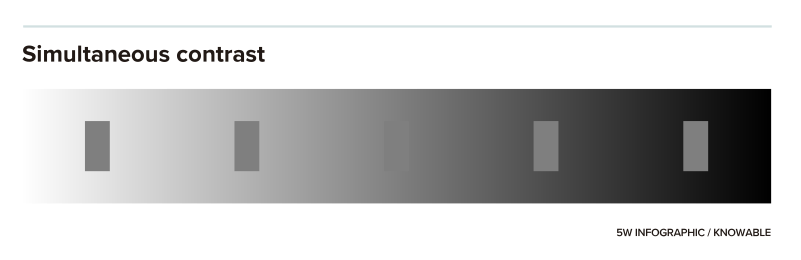
\includegraphics[width=\textwidth]{../figures/plotting_gray_scale_clustering.pdf}
	\end{center}
\end{frame}

\begin{frame}
	\frametitle{Color Contrasts}
	\vspace{-0.25cm}
	\begin{center}
		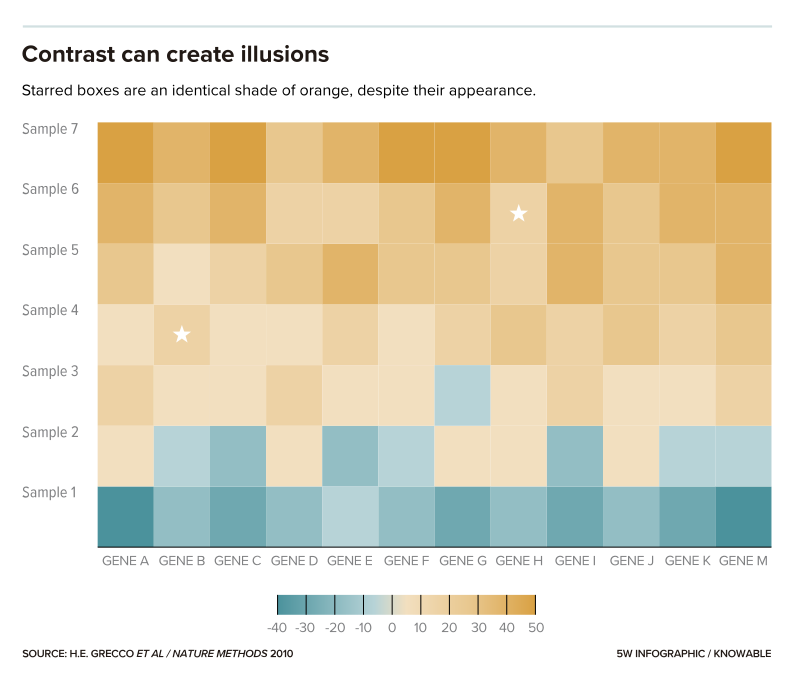
\includegraphics[width=.8\textwidth]{../figures/plotting_color_clustering.pdf}
	\end{center}
\end{frame}


\begin{frame}
	\frametitle{Plotting Tools}
	\begin{itemize}
		\item There are many tools. 
		\item Don't get limited by the tools / defaults
		\item Invest some time to research which tool helps you realize the vision for your data visualization
		\item Program your own graphics if necessary (Python, GMT, 3djs, \dots)
	\end{itemize}
\end{frame}

\begin{frame}
	\frametitle{Plotting Tools}
	Python:
	\begin{center}
		\hspace{4cm}\includegraphics[width=.49\textwidth]{../figures/seaborn_logo.pdf}
	\end{center}
	\begin{center}
		\vspace{-0.75cm}
		\hspace{-4cm}\includegraphics[width=.49\textwidth]{../figures/matplotlib_logo.pdf}
	\end{center}
	
	Unix:
	\begin{center}
		\hspace{-4cm}\includegraphics[width=.49\textwidth]{../figures/gmt_logo.png}
	\end{center}
	\begin{center}
		\vspace{-0.75cm}
		\hspace{6cm}\includegraphics[width=.49\textwidth]{../figures/python_logo.pdf}
	\end{center}
\end{frame}


\begin{frame}
	\frametitle{Matplotlib}
	\begin{block}{pyplot API}
	matplotlib.pyplot is intended for simple cases of programmatic plot generation, it provides a set of 
	functions that make Matplotlib work like MATLAB. 
	\end{block}

	\begin{block}{object-oriented API}
	If you need more control and customization, work directly with the figure objects that matplotlib generates
	\end{block}
\end{frame}

\begin{frame}
	\frametitle{matplotlib.pyplot}
	\vspace{-0.25cm}
	\begin{center}
		\includegraphics[width=.7\textwidth]{../figures/matplotlib_pyplot.png}
	\end{center}
	\begin{flushright}
		\vspace{-1cm}
		\tiny{\emph{matplotlib.org}}
	\end{flushright}
\end{frame}

\begin{frame}
	\frametitle{Matplotlib Figure Anatomy}
	\vspace{-0.25cm}
	\begin{center}
		\includegraphics[width=.65\textwidth]{../figures/matplotlib_figure_anatomy.png}
	\end{center}
	\begin{flushright}
		\vspace{-1cm}
		\tiny{\emph{matplotlib.org}}
	\end{flushright}
\end{frame}

%\begin{frame}
%	\frametitle{Matplotlib - maps (Geopandas)}
%\end{frame}

\begin{frame}
	\frametitle{Seaborn}
	\vspace{-0.25cm}
	\begin{center}
		\includegraphics[width=\textwidth]{../figures/seaborn_figures.png}
	\end{center}
	\begin{flushright}
		\vspace{-0.25cm}
		\tiny{\emph{seaborn.pydata.org}}
	\end{flushright}

	\begin{block}{}
	``Seaborn is a library for making statistical graphics in Python. It builds on top of matplotlib and integrates closely with pandas data structures.``
	\end{block}
\end{frame}


\end{document}
